\documentclass{standalone}
\usepackage{tikz}
\usetikzlibrary{patterns, positioning}


\begin{document}
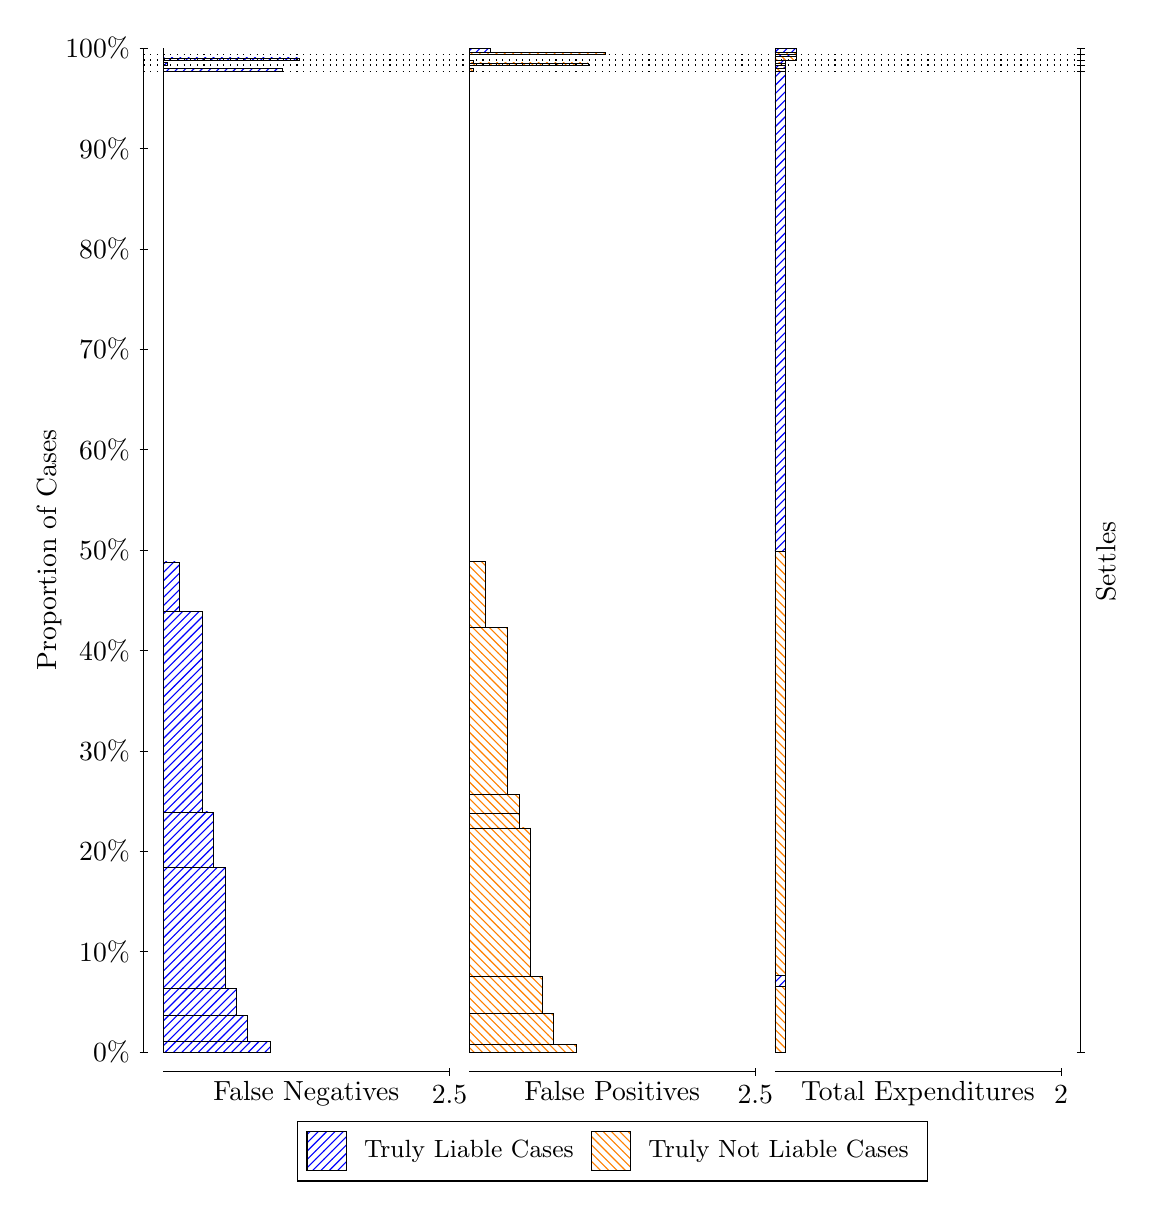
\begin{tikzpicture}
\draw[black, very thin] (1.5,1.75) -- (1.5,14.5);
\node[rotate=90, text=black, anchor=center] at (0.3, 8.125) {Proportion of Cases};
\draw[black, very thin] (1.45,1.75) -- (1.55,1.75);
\node[text=black, anchor=east] at (1.45, 1.75) {0\%};
\draw[black, very thin] (1.45,3.025) -- (1.55,3.025);
\node[text=black, anchor=east] at (1.45, 3.025) {10\%};
\draw[black, very thin] (1.45,4.3) -- (1.55,4.3);
\node[text=black, anchor=east] at (1.45, 4.3) {20\%};
\draw[black, very thin] (1.45,5.575) -- (1.55,5.575);
\node[text=black, anchor=east] at (1.45, 5.575) {30\%};
\draw[black, very thin] (1.45,6.85) -- (1.55,6.85);
\node[text=black, anchor=east] at (1.45, 6.85) {40\%};
\draw[black, very thin] (1.45,8.125) -- (1.55,8.125);
\node[text=black, anchor=east] at (1.45, 8.125) {50\%};
\draw[black, very thin] (1.45,9.4) -- (1.55,9.4);
\node[text=black, anchor=east] at (1.45, 9.4) {60\%};
\draw[black, very thin] (1.45,10.675) -- (1.55,10.675);
\node[text=black, anchor=east] at (1.45, 10.675) {70\%};
\draw[black, very thin] (1.45,11.95) -- (1.55,11.95);
\node[text=black, anchor=east] at (1.45, 11.95) {80\%};
\draw[black, very thin] (1.45,13.225) -- (1.55,13.225);
\node[text=black, anchor=east] at (1.45, 13.225) {90\%};
\draw[black, very thin] (1.45,14.5) -- (1.55,14.5);
\node[text=black, anchor=east] at (1.45, 14.5) {100\%};

\draw[black, very thin] (13.4,1.75) -- (13.4,14.5);
\draw[black, very thin] (13.35,1.75) -- (13.45,1.75);
\node[anchor=west] at (13.35, 1.75) {};
\draw[black, very thin] (13.35,14.201) -- (13.45,14.201);
\node[anchor=west] at (13.35, 14.201) {};
\draw[black, very thin] (13.35,14.284) -- (13.45,14.284);
\node[anchor=west] at (13.35, 14.284) {};
\draw[black, very thin] (13.35,14.348) -- (13.45,14.348);
\node[anchor=west] at (13.35, 14.348) {};
\draw[black, very thin] (13.35,14.423) -- (13.45,14.423);
\node[anchor=west] at (13.35, 14.423) {};
\draw[black, very thin] (13.35,14.5) -- (13.45,14.5);
\node[anchor=west] at (13.35, 14.5) {};

\draw[black, very thin, pattern color=blue, pattern=north east lines] (1.75,1.75) rectangle (3.1125,1.8839);
\draw[black, very thin, pattern color=blue, pattern=north east lines] (1.75,1.8839) rectangle (2.8218,2.2145);
\draw[black, very thin, pattern color=blue, pattern=north east lines] (1.75,2.2145) rectangle (2.6765,2.5597);
\draw[black, very thin, pattern color=blue, pattern=north east lines] (1.75,2.5597) rectangle (2.5312,4.0936);
\draw[black, very thin, pattern color=blue, pattern=north east lines] (1.75,4.0936) rectangle (2.3858,4.7999);
\draw[black, very thin, pattern color=blue, pattern=north east lines] (1.75,4.7999) rectangle (2.2405,7.3476);
\draw[black, very thin, pattern color=blue, pattern=north east lines] (1.75,7.3476) rectangle (1.9498,7.9737);
\draw[black, very thin, pattern color=orange, pattern=north west lines] (1.75,7.9737) rectangle (1.75,14.201);
\draw[black, very thin, pattern color=blue, pattern=north east lines] (1.75,14.201) rectangle (3.2578,14.238);
\draw[black, very thin, pattern color=orange, pattern=north west lines] (1.75,14.238) rectangle (1.75,14.284);
\draw[black, very thin, pattern color=blue, pattern=north east lines] (1.75,14.284) rectangle (1.8045,14.321);
\draw[black, very thin, pattern color=orange, pattern=north west lines] (1.75,14.321) rectangle (1.75,14.348);
\draw[black, very thin, pattern color=blue, pattern=north east lines] (1.75,14.348) rectangle (3.4758,14.374);
\draw[black, very thin, pattern color=orange, pattern=north west lines] (1.75,14.374) rectangle (1.75,14.423);
\draw[black, very thin, pattern color=orange, pattern=north west lines] (1.75,14.423) rectangle (1.75,14.449);
\draw[black, very thin, pattern color=blue, pattern=north east lines] (1.75,14.449) rectangle (1.75,14.5);
\draw[black, very thin, pattern color=orange, pattern=north west lines] (5.6333,1.75) rectangle (6.9958,1.8502);
\draw[black, very thin, pattern color=orange, pattern=north west lines] (5.6333,1.8502) rectangle (6.7052,2.2365);
\draw[black, very thin, pattern color=orange, pattern=north west lines] (5.6333,2.2365) rectangle (6.5598,2.707);
\draw[black, very thin, pattern color=orange, pattern=north west lines] (5.6333,2.707) rectangle (6.4145,4.5952);
\draw[black, very thin, pattern color=orange, pattern=north west lines] (5.6333,4.5952) rectangle (6.2692,4.7768);
\draw[black, very thin, pattern color=orange, pattern=north west lines] (5.6333,4.7768) rectangle (6.2692,5.019);
\draw[black, very thin, pattern color=orange, pattern=north west lines] (5.6333,5.019) rectangle (6.1238,7.1423);
\draw[black, very thin, pattern color=orange, pattern=north west lines] (5.6333,7.1423) rectangle (5.8332,7.9777);
\draw[black, very thin, pattern color=blue, pattern=north east lines] (5.6333,7.9777) rectangle (5.6333,14.201);
\draw[black, very thin, pattern color=orange, pattern=north west lines] (5.6333,14.201) rectangle (5.6878,14.247);
\draw[black, very thin, pattern color=blue, pattern=north east lines] (5.6333,14.247) rectangle (5.6333,14.284);
\draw[black, very thin, pattern color=orange, pattern=north west lines] (5.6333,14.284) rectangle (7.1412,14.311);
\draw[black, very thin, pattern color=blue, pattern=north east lines] (5.6333,14.311) rectangle (5.6878,14.348);
\draw[black, very thin, pattern color=orange, pattern=north west lines] (5.6333,14.348) rectangle (5.6333,14.396);
\draw[black, very thin, pattern color=blue, pattern=north east lines] (5.6333,14.396) rectangle (5.6333,14.423);
\draw[black, very thin, pattern color=orange, pattern=north west lines] (5.6333,14.423) rectangle (7.3592,14.449);
\draw[black, very thin, pattern color=blue, pattern=north east lines] (5.6333,14.449) rectangle (5.9058,14.5);
\draw[black, very thin, pattern color=orange, pattern=north west lines] (9.5167,1.75) rectangle (9.6529,2.5854);
\draw[black, very thin, pattern color=blue, pattern=north east lines] (9.5167,2.5854) rectangle (9.6529,2.7193);
\draw[black, very thin, pattern color=orange, pattern=north west lines] (9.5167,2.7193) rectangle (9.6529,8.1116);
\draw[black, very thin, pattern color=blue, pattern=north east lines] (9.5167,8.1116) rectangle (9.6529,14.201);
\draw[black, very thin, pattern color=orange, pattern=north west lines] (9.5167,14.201) rectangle (9.6529,14.247);
\draw[black, very thin, pattern color=blue, pattern=north east lines] (9.5167,14.247) rectangle (9.6529,14.284);
\draw[black, very thin, pattern color=orange, pattern=north west lines] (9.5167,14.284) rectangle (9.6529,14.311);
\draw[black, very thin, pattern color=blue, pattern=north east lines] (9.5167,14.311) rectangle (9.6529,14.348);
\draw[black, very thin, pattern color=orange, pattern=north west lines] (9.5167,14.348) rectangle (9.7892,14.396);
\draw[black, very thin, pattern color=blue, pattern=north east lines] (9.5167,14.396) rectangle (9.7892,14.423);
\draw[black, very thin, pattern color=orange, pattern=north west lines] (9.5167,14.423) rectangle (9.7892,14.449);
\draw[black, very thin, pattern color=blue, pattern=north east lines] (9.5167,14.449) rectangle (9.7892,14.5);
\draw[black, dotted] (1.5,14.201) -- (13.4,14.201);
\draw[black, dotted] (1.5,14.284) -- (13.4,14.284);
\draw[black, dotted] (1.5,14.348) -- (13.4,14.348);
\draw[black, dotted] (1.5,14.423) -- (13.4,14.423);
\draw[black, very thin] (1.75,1.5) -- (5.3833,1.5);
\node[text=black, anchor=north] at (3.5667, 1.5) {False Negatives};
\draw[black, very thin] (5.3833,1.45) -- (5.3833,1.55);
\node[text=black, anchor=north] at (5.3833, 1.45) {2.5};

\draw[black, very thin] (5.6333,1.5) -- (9.2667,1.5);
\node[text=black, anchor=north] at (7.45, 1.5) {False Positives};
\draw[black, very thin] (9.2667,1.45) -- (9.2667,1.55);
\node[text=black, anchor=north] at (9.2667, 1.45) {2.5};

\draw[black, very thin] (9.5167,1.5) -- (13.15,1.5);
\node[text=black, anchor=north] at (11.333, 1.5) {Total Expenditures};
\draw[black, very thin] (13.15,1.45) -- (13.15,1.55);
\node[text=black, anchor=north] at (13.15, 1.45) {2};

\node[text=black, centered, rotate=90] at (13.72, 7.9757) {Settles};





\draw (7.449999999999999,1.5) node[draw=none] (baseCoordinate) {};
\begin{scope}[align=center]
        \matrix[scale=0.5, draw=black, below=0.5cm of baseCoordinate, nodes={draw}, column sep=0.1cm]{
            \node[rectangle, draw, minimum width=0.5cm, minimum height=0.5cm, pattern color=blue, pattern=north east lines] {}; &
            \node[draw=none, font=\small, text=black] (B) {Truly Liable Cases}; &
            \node[rectangle, draw, minimum width=0.5cm, minimum height=0.5cm, pattern color=orange, pattern=north west lines] {}; &
            \node[draw=none, font=\small, text=black] (B) {Truly Not Liable Cases}; \\
            };
\end{scope}

\end{tikzpicture}
\end{document}